\documentclass[tikz, border=2mm]{standalone}
\usepackage{amsmath}
\usetikzlibrary{automata, positioning, arrows}
\tikzset{
  ->, % makes the edges directed
  >=stealth', % makes the arrow heads bold
  node distance=3cm, % specifies the minimum distance between two nodes. Change if necessary.
  every state/.style={thick}, % sets the properties for each ’state’ node
  initial text=, % sets the text that appears on the start arrow
}

\begin{document}

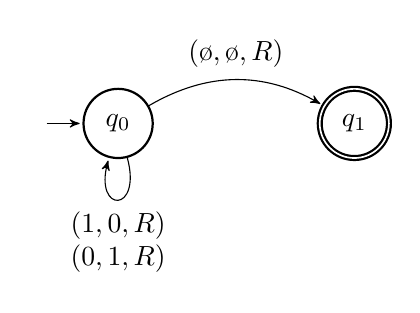
\begin{tikzpicture}[shorten >=1pt, on grid, auto]
  \node[state, initial] (0) {$q_0$};
  \node[state, right of=0, accepting] (1) {$q_1$};
  
   \draw (0) edge[loop below] node[below]{$
    \begin{aligned}
      (1, 0, R)\\[-0.7ex]
      (0, 1, R)
    \end{aligned}$} (0);
     
    
  \draw  
    (0) edge[bend left, above] node[above]{$
    \begin{aligned}
      (\o{}, \o{}, R)
    \end{aligned}$} (1);      

 
\end{tikzpicture}

\end{document}